\documentclass[letterpaper,12pt]{article}

\usepackage{fullpage}
\usepackage{fancyhdr}
\usepackage{xcolor}
\usepackage{hyperref}
\definecolor{linkcolour}{rgb}{0,0.2,0.6}
\hypersetup{colorlinks,breaklinks,urlcolor=linkcolour, linkcolor=linkcolour}
%\hyperref[label_name]{''link text''}


\usepackage{array}
\usepackage{tabularx}
\usepackage[english]{babel}
\usepackage{multirow}
\usepackage{booktabs}
\usepackage{mathrsfs}
\usepackage{setspace}
%\usepackage{lineno}
\usepackage{subfigure}
\usepackage{mathrsfs}
\usepackage{amsmath}
\usepackage{cite}
\usepackage{comment}
\usepackage{rotating}
\usepackage{array}
\usepackage{comment}

\usepackage{lmodern}
\usepackage[T1]{fontenc} 
\usepackage[latin1]{inputenc} 
\usepackage{textcomp}
%\usepackage{lineno}

%\usepackage{pygmentize}
%\usepackage{times}
\usepackage{xcolor}
\usepackage{listings}

\colorlet{mygray}{black!30}
\colorlet{mygreen}{green!60!blue}
\colorlet{mymauve}{red!60!blue}

\lstset{
  backgroundcolor=\color{gray!10},  
  basicstyle=\ttfamily,
  columns=fullflexible,
 % breakatwhitespace=false,      
  breaklines=true,                
 % captionpos=b,                    
  commentstyle=\color{mygreen}, 
  %extendedchars=true,              
  frame=single,                   
  % keepspaces=true,             
  keywordstyle=\color{blue},      
  language=c++,                 
  numbers=none,                
  numbersep=5pt,                   
  numberstyle=\tiny\color{blue}, 
  rulecolor=\color{mygray},        
  % showspaces=false,               
  % showtabs=false,                 
  stepnumber=4,                  
  stringstyle=\color{mymauve},    
  tabsize=3,                      
  title=\lstname                
}

\usepackage{url,parskip} 	%other packages for formatting
%\usepackage{minted}
\newcommand{\HRule}{\rule[20pt]{\linewidth}{0.3mm}}
\newcommand{\HRulesmall}{\rule[10pt]{0.5\linewidth}{0.3mm}}
\newcommand{\atlas}{{\sc Atlas}}
\newcommand{\cdf}{{\sc CDF}}
\newcommand{\TeV}{{Te\kern -0.1em V}}
\newcommand{\tev}{{Te\kern -0.1em V}}
\newcommand{\GeV}{{Ge\kern -0.1em V}}
\newcommand{\gev}{{Ge\kern -0.1em V}}
%\def\TeV{\ifmmode {\mathrm{\ Te\kern -0.1em V}}\else
%                   \textrm{Te\kern -0.1em V}\fi}%
\newcommand{\trileptoncdf}{\ensuremath{p\bar{p}\rightarrow \tilde{\chi}_2^0\tilde{\chi}_1^\pm \rightarrow \ell\ell\ell\nu\tilde{\chi}_1^0\tilde{\chi}_1^0  }}
\newcommand{\cnlep}{\ensuremath{\tilde{\chi}_2^0\tilde{\chi}_1^\pm \rightarrow \ell^+\ell^-\ell^\pm\nu\tilde{\chi}_1^0\tilde{\chi}_1^0}}
\newcommand{\dchlep}{\ensuremath{H^{++}H^{--}\rightarrow \ell^{+}\ell^{+}\ell^{-}\ell^{-} }}
\newcommand{\bprimelep}{\ensuremath{b'\bar{b}' \rightarrow WtWt \rightarrow WWbWWb}}
\def\ifb{\mbox{fb$^{-1}$ }}%  Inverse femtobarns.

\addtolength\topmargin{-1cm}
%\addtolength\oddsidemargin{-1cm}
%\addtolength\evensidemargin{-1cm}
%\addtolength\textwidth{2cm}
\addtolength\textheight{2cm}

%\setlength\oddsidemargin{1cm}
%\setlength\evensidemargin{1cm}

\newcounter{pubcount}

\include{definitions}



\begin{document}

%\linenumbers

%\pagestyle{empty} % non-numbered pages
\pagestyle{fancy}
\fancyhead{}
\fancyfoot{}
\renewcommand{\headrulewidth}{0.pt}
\renewcommand{\footrulewidth}{0.pt}
\fancyfoot[RO, RE] {\thepage{}}
\fancyfoot[LO, LE] {{ROOT tutorial}}

\vspace*{2mm}

\thispagestyle{empty}
\begin{center}
\Large{\sc  Welcome package - week 3\\}
\vspace*{2mm}

\large{\sc ROOT Tutorial}  
\end{center}
\vspace*{3mm}
\begin{tabular*}{\linewidth}{l@{\extracolsep{\fill}}r}
   \normalsize{} &\normalsize{Sreelakshmi Sindhu, Ishan Pokharel, Chris Scheulen}\\
%    \small{Indian Institute of Science Education and Research, Pune} &\small{Goerg-August-Universitaet Goettingen}\\
 
\end{tabular*}% 
\vspace*{3mm}
\HRule
\vspace*{-2.5mm}


\section{Introduction}
\label{sec:intro}
Aim of this tutorial is to give you a first hand experience on using root to perform some basic data analysis that will come in use during your Bachelor thesis. Today we will start with the first part which includes, reading event attributes from a TTree, filling it to a histogram and writing it to an output file. 

\section{Writing a ROOT macro}
\begin{itemize}
\item {\bf Step 1: Creating the outline}
\begin{itemize}
	\item The main function in a ROOT macro should have the same name as the file name. For example, if your file name is EventLoopExample.cxx" the the main function should be called EventLoopExample() 

	\item Within the macro the main function can look something like this:
	 \begin{lstlisting}
	void EventLoopExample()
	 	{
	 	std::cout << "Testing my ROOT macro" << std::endl;
	 	}

\end{lstlisting}
	\item Run the macro using ROOT:
\begin{verbatim}
root -l "EventLoopExample.cxx"
	\end{verbatim}
		\item Also, include appropriate header files of ROOT classes you will use. For Example:
		\begin{lstlisting}
		#include "TFile.h"
		\end{lstlisting}
	\end{itemize} 	

	\item {\bf Step 2: Set the input and output arguments}\\
	\begin{itemize}
	
		\item We want the macro to read the input file: "/afs/cern.ch/user/i/ispokhar/pub lic/sampleNtuple/" and store the information that we need in a new file.
		\item Declare the input file path and the output file path. For Example:
			\begin{lstlisting}

	void EventLoopExample()
	 	{
	 	
	 	std::string pathToInputFile = "";
	 	std::string pathToOutputFile = "";
		std::cout << "Reading from " << pathToInputFile <<
		 " and writing to " << pathToOutputFile << std::endl;
	 	
	 	}

\end{lstlisting}




\item Declare TChain and add the file to the TChain.  
			\begin{lstlisting}
	TChain Chain_A("nominal");
\end{lstlisting}
\item Read events from the nominal tree.
\begin{lstlisting}
	Chain_A.Add(pathToInputFile);

\end{lstlisting}
\end{itemize}
\item {\bf Step 3: Identifying the variables, declaring them and setting branch address}\\
 Next we have to identify the branch address for the variables we are interested in and link their branch address. For example, for the photon $p_{T}$ : 
\begin{itemize}
\item Declare a variable that will hold the object kinematics as a pointer: (make sure that the datatype is matched)
\begin{lstlisting}
	std::vector<float> *v_pt_A =0;
\end{lstlisting}
\item Declare the branch that holds the information in the ntuple:
\begin{lstlisting}
	TBranch *b_pt_A =0;
\end{lstlisting}

\item Now link the branch to the variable where the information has to be stored temporarily, using TTree::SetBranchAddress. %Here, "ph\_pt" is the name of the branch.
\begin{lstlisting}
	Chain_A.SetBranchAddress("ph_pt", &v_pt_A, &b_pt_A);
\end{lstlisting}
\end{itemize}
\item {\bf Step 4: Declare histograms:}
\begin{itemize}
\item Our aim is to store the information from the ntuple to a histogram. For that first we have to declare them as TH1 objects:
 \begin{lstlisting}
 TH1F* pt_A = new TH1F("A_pt", "", 20, 0, 400);
\end{lstlisting}
\item Here the arguments are as follows: (name of the histogram, title of the histogram, number of bins, starting point of first bin, ending point of last bin)
	\end{itemize}
\item {\bf Step 5: Loop over the events}
\begin{itemize}

\item Now write a simple loop over all events.
\item Within the loop fill the histograms
\item Event information can be obtained within the loop using:
\begin{lstlisting}
	Chain_A.GetEntry(ievent);
\end{lstlisting}
\item The number of events in the tree can be accessed using:

\begin{lstlisting}
int entries_A = Chain_A.GetEntries();
\end{lstlisting}
\end{itemize}
\item {\bf Step 6: Write the histogram to output file}
\begin{itemize}
	\item The final step is to create a TFile to store the histogram. 
\item cd() into the file $\rightarrow$ Write the histogram $\rightarrow$Close the file

\begin{lstlisting}     
TFile* outFile = new TFile(outPath + "outFile.root", "RECREATE");
outFile->cd();             
pt_A->Write("pt_A");
outFile->Close();                                                    
         \end{lstlisting}
\end{itemize}

\item{\bf Step 7: Additional assignments}
\begin{itemize}
	\item Write more histograms to the TFile: Specifically, add, "ph\_eta" and "ph\_phi".  
	\item Fill a 2D Histogram with photon $p_{T}$ on x-axis and $\eta$ on the y-axis.
	\begin{lstlisting}
 TH2F* hist2D_A = new TH2F("pTvsEta_A", "", 20, 0, 400, 20, -2.5, 2.5);
\end{lstlisting}

\item Add another input file: "/eos/user/a/ankirchh/ttgamma-analysis/mini-n\
tuples/ljets/mc16d\_TOPQ1\_ttgamma\_LO\_dec.412114.root" \\
This file contains events with FSR photons. The file you worked with till now contains $t\bar{t}\gamma$ events with ISR photons.\\ 


\begin{figure}[h]
  \centering
  \subfigure[Photon radiated from the initial state particle (ISR)]{
  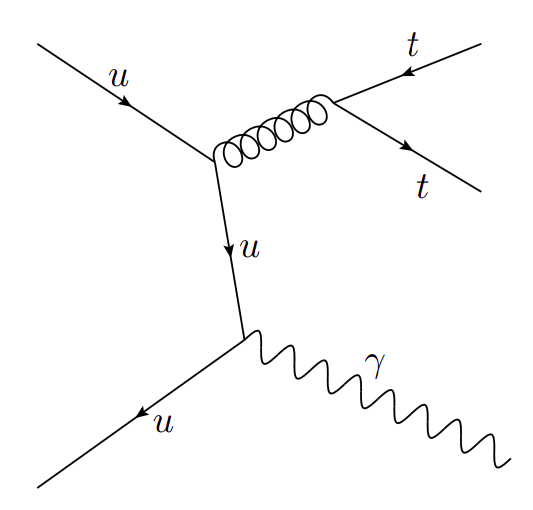
\includegraphics[width=0.33\textwidth]{isr.png}}
  % \subfigure[from top quark]{
  % 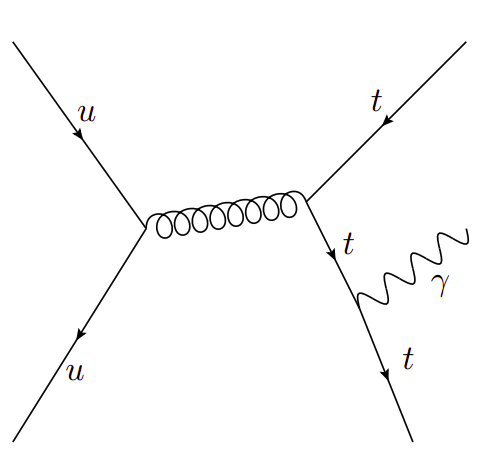
\includegraphics[width=0.2\textwidth]{top.png}}
   \subfigure[Photon radiated from final state particle (FSR)]{
   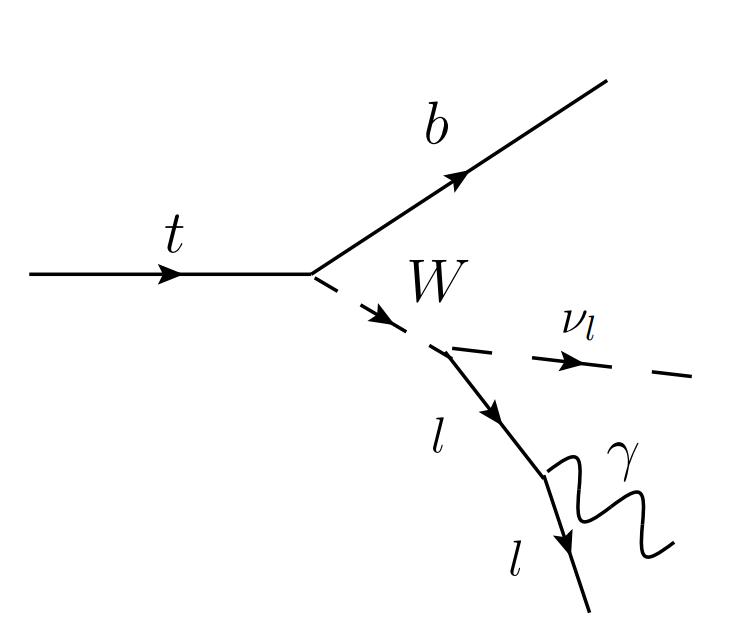
\includegraphics[width=0.33\textwidth]{fsr.png}}
  \caption{Feynman diagrams of $t\bar{t}\gamma$ production}
  \label{fig:tty}
\end{figure}

\item Add another event loop and write, "ph\_pt", "ph\_eta" and "ph\_phi" for the FSR photons to the same TFile.   
\end{itemize}
\item Outlook: These histograms will be used in tomorrow's session.
\end{itemize}
\break
\section{Plotting using PYROOT}

In this session we will focus on plotting these histograms and saving them as png/pdf files. It is usually useful to overlay histograms and take ratios to do some comparative study. We will use PYROOT to do this in this session but this can also be done using ROOT based on C++. 

\subsection{Making a simple plot}
First access the root file that we created using Tfile and get the required histogram using the Get command. Create a canvas, now draw the histogram using the Draw option ans Save the file. A simple example is below:

\begin{lstlisting}
import ROOT
from ROOT import TCanvas, TFile

Hist_file = TFile("path_to_file")
Hist_name = Hist_file.Get("name_of_the_histogram")
canvas = TCanvas("name", "title", width, height)
Hist_name.Draw("HIST")
canvas.SaveAs("file_name.pdf")

\end{lstlisting}

\subsection{Making it presentable}
The plots can be made easier to understand by adding axis-labels, titles, picking colours and adding texts. These can be done using  using TLegend, TGaxis, TColor, TH1F, TPad.. Remember to import appropriate header files for each of these classes. 
Details on the arguments required can be found in the \href{https://root.cern/doc/master/}{reference guide}. Some examples:

\begin{lstlisting}
Hist_name.GetYaxis().SetTitle("Events")
\end{lstlisting}

\subsection{Making ratio plots}
You can make several pads within the canvas using TPad. An additional pad can be added for showing the ratio plot.  
%\subsection{Setting up atlasplots}

\section{Performing a fit}
%This will be done using EFT\textit{fitter}\cite{eftfitter} tool.
% \bibliography{bibtex_file}
% \bibliographystyle{bthesis}

%% \begin{thebibliography}{10}

%% \bibitem{prlfb}
%%   O. ~Bylund {\it et al.}  [CDF Collaboration],
%%   Phys.\ Rev.\ Lett.\  {\bf 101}, 251801 (2008)
%%   [arXiv:0808.2446 [hep-ex]].

%% \bibitem{cdfprl}
%%   T.~Aaltonen {\it et al.}  [CDF Collaboration],
%%   Phys.\ Rev.\ Lett.\  {\bf 99}, 191806 (2007)
%%   [arXiv:0707.2362 [hep-ex]].


%% \bibitem{smeft}
%%   Bylund, O.B., Maltoni, F., Tsinikos, I. et al. J. High Energ. Phys. (2016) 2016: 52. https://doi.org/10.1007/JHEP05(2016)052.

%% \bibitem{smeft2}
%%   Hartland, N.P., Maltoni, F., Nocera, E.R. et al. J. High Energ. Phys. (2019) 2019: 100. https://doi.org/10.1007/JHEP04(2019)100
%% \bibitem{mg}
%%   Alwall, J., Frederix, R., Frixione, S. et al. J. High Energ. Phys. (2014) 2014: 79. https://doi.org/10.1007/JHEP07(2014)079


%% \end{thebibliography}


\end{document}
